\documentclass[a4paper,11pt,dvipdfmx]{ujarticle}
% パッケージ
\usepackage{graphicx}
\usepackage{url}
% レイアウト指定を記述したファイルの読み込み
\input{layout}

% タイトルと氏名を変更せよ.
\title{日本におけるデジタル化の状況}
\author{G584502025 佐藤真優}

\begin{document}

\maketitle %ここにタイトルが入る

% ここから本文
% 節見出し: \section{}
% を使う
\section{デジタル競争力ランキング}
% 本文(1)
%  参考文献の参照: \cite{}
%  図番号の参照: \ref{}
% を使う
% 文献データベースのキーワードは oecd と imd
% になっている.
国際経営開発研究所(IMD)の調査\cite{IMD}によると,
日本のデジタル競争力ランキングは図\ref{fig:競争力}に示すように,
調査対象の64カ国中、総合で28位、準備分野で27位となっている。
% 図の挿入
% \includegraphics{}
% を
% \begin{figure}[htbp]
% \end{figure}
% で囲み
% \caption{}
% で図のタイトルを入れる.
% \label{}
% を使って図番号が参照できるようにする
% また,
% \centering
% で図が中央に来るようにする
\begin{figure}[htbp]
    \centering
    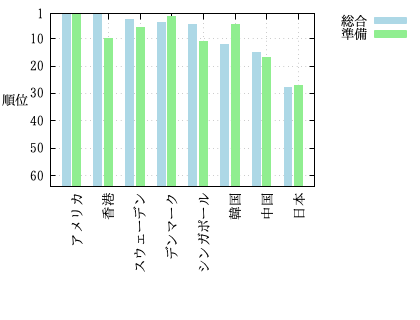
\includegraphics{fig51.png}
    \caption{デジタル競争力ランキング(64カ国中)}\label{fig:競争力}
\end{figure}
% ーーー
% 節見出し(2)
\section{ブロードバンドの整備状況}
% 本文(2)
OECDによるブロードバンド回線の普及に関する調査\cite{oecd}によると、
表\ref{tbl:加入者数}に示すように、日本における100人あたりの光ファイバー回線の加入者は39.0で
韓国、スウェーデン、ノルウェーに続いて第4位になっている。
% 表の挿入
% \begin{tabular}
% \end{tabular}    
% による表の記述を 
% \begin{table}[htbp]
% \end{table}
% で囲み
% \caption{}
% で表のタイトルを入れる.
% \label{}
% を使って表番号が参照できるようにする
% また,
% \centering
% で表が中央に来るようにする
\begin{table}[http]
    \centering
    \caption{光ファイバー回線の加入者(100人あたり)}
    \label{tbl:加入者数}

    \begin{tabular}{|l|r|r|}\hline
        順位 & 国名 & 加入者数(\%) \\
        \hline
        1位 & 韓国 & 38.2 \\
        \hline
        2位 & 従来型の携帯電話 & 7.0 \\
        \hline
        3位 & タブレット & 26.5 \\
        \hline
        4位 & ノートPC & 48.5 \\
        \hline
        5位 & デスクトップPC & 20.9 \\
        \hline
        6位 & ゲーム機 & 11.4 \\
        \hline 
        7位 & テレビ & 50.8 \\
        \hline
        8位 & ニュージーランド & 23.6 \\
        \hline
        9位 & リトアニア & 22.3 \\
        \hline
        10位 & フランス & 21.2 \\
        \hline
    \end{tabular}
\end{table}
% ーーー
% 見出し(3)
% 考察
\section{考察}
% \begin{itemize}
% \end{itemize}
% を使って箇条書きで記述する
\begin{itemize}
    \item デジタル競争力ランキングの日本の順位が低いことから教育や政策支援などに課題があると考察される。
    \item シンガポールや韓国は高順位。このことからデジタル分野での戦略が結果を出していると考えられる。
    \item 韓国が一位であることは先進国であることがわかる。このことから都心部を中心とした集中整備や、政府の推進策が結果を出していると考えられる。
\end{itemize}
% ここに参考文献が入る
%
\bibliographystyle{junsrt}
\bibliography{exercise.bib}

\end{document}